\section{Praxis Beispiele}
\subsection{Optik}
Gilt nur für sehr kleine Winkel (Annahme: $\sin\alpha \approx \alpha \approx \tan\alpha$). Die entgültige Optik-Matrix ist eine Multiplikationen von allen Brechungen. \\


\begin{minipage}{\textwidth}
	\noindent Beschreibung eines Lichtstrahls:
	
	\begin{minipage}{0.25\textwidth}
		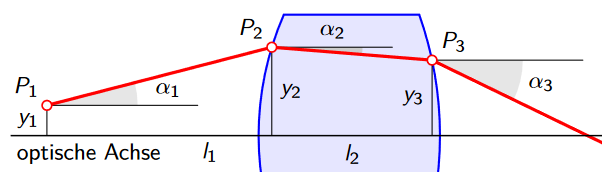
\includegraphics[width=\linewidth,keepaspectratio=true]{./Images/optik_lichstrahl.png}
	\end{minipage}%%% to prevent a space
	\begin{minipage}{0.25\textwidth}	
		\[
			\underbrace{\begin{pmatrix} 1 & l \\ 0 & 1\end{pmatrix}}_{T_{\text{Weg}}(l)}
			\underbrace{\begin{pmatrix} y \\ \alpha \end{pmatrix}}_{StartStrahl}
		\]
	\end{minipage}
\end{minipage}

\begin{minipage}{\textwidth}
	\noindent Brechung an einer Kugeloberfläche:
	
	\begin{minipage}{0.25\textwidth}
		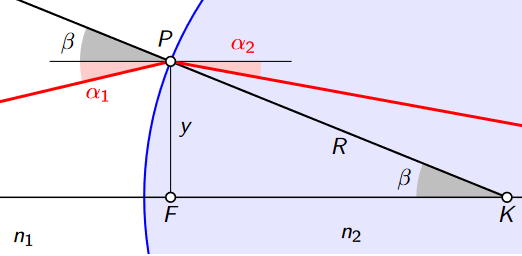
\includegraphics[width=\linewidth,keepaspectratio=true]{./Images/optik_kugel.png}
	\end{minipage}%%% to prevent a space
	\begin{minipage}{0.25\textwidth}	
		\[
		\underbrace{
			\begin{pmatrix}
				1 & 0\\
				\frac{1}{R}\left(\frac{n_1}{n_2} - 1\right) & \frac{n_1}{n_2}
			\end{pmatrix}
		}_{T_{\text{Brechung}}(n_1,n_2,R)}
		\]
	\end{minipage}
\end{minipage}

\begin{minipage}{\textwidth}
	\noindent Brennweite:
	
	\begin{minipage}{0.25\textwidth}
		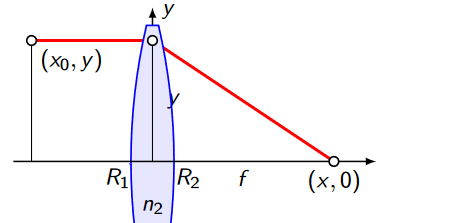
\includegraphics[width=\linewidth,keepaspectratio=true]{./Images/optik_brennweite.png}
	\end{minipage}%%% to prevent a space
	\begin{minipage}{0.25\textwidth}	
		\[\underbrace{
			\begin{pmatrix} 
				1 & 0 \\ 
				-\frac{1}{f} & 1
			\end{pmatrix}
		}_{T_{\text{Linse}}(f)}
		\]
	\end{minipage}
\end{minipage}

\noindent \textbf{Beispiel}:\\
\begin{center}
	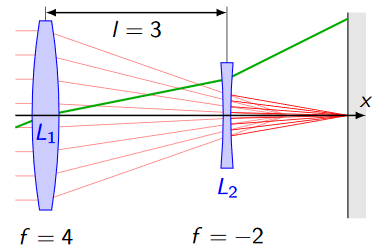
\includegraphics[height=10em]{./Images/optik_beispiel.png}
\end{center}

\begin{align*}
	T_{\text{Linse}_1}(4) &= \begin{pmatrix}
		1 & 0 \\ -\frac{1}{4} & 1
	\end{pmatrix} \quad 
	T_{\text{Weg}}(3) &= \begin{pmatrix}
		1 & 3 \\ 0 & 1
	\end{pmatrix} \\
	T_{\text{Linse}_2}(-2) &= \begin{pmatrix}
		1 & 0 \\ \frac{1}{2} & 1
	\end{pmatrix}
\end{align*}

\noindent Das System wird von \underline{rechts nach links} beschrieben. Daraus ergibt sich folgende Multiplikation:
\[
\underbrace{
	\begin{pmatrix}
		1 & x \\ 0 & 1
	\end{pmatrix}
}_{T_{\text{Weg}}}
\overbrace{
	\underbrace{
		\begin{pmatrix}
			1 & 0 \\ \frac{1}{2} & 1
		\end{pmatrix}
	}_{T_{\text{Linse}_2}}
	\underbrace{
		\begin{pmatrix}
			1 & 3 \\ 0 & 1
		\end{pmatrix}
	}_{T_{\text{Weg}}}
	\underbrace{
		\begin{pmatrix}
			1 & 0 \\ -\frac{1}{4} & 1
		\end{pmatrix}
	}_{T_{\text{Linse}_1}}
}^{T}
\underbrace{
	\begin{pmatrix}
		1 \\ 0
	\end{pmatrix}
}_{\text{StartStrahl}}
\]

\subsection{Potenzen}\label{potenz}
Um eine Potenz einer Matrix zu berechnen wird die Matrix $A$ diagonalisiert zu $A'$. Anschliessend wird $A'^k$ berechnet und wieder zurück in die Ursprüngliche Basis transformiert.

\[ A^k = T^{-1}A'^kT \]

\noindent Beispiel:
\[ 
A = \begin{pmatrix}
	3 & 2 \\ 1 & 2
\end{pmatrix}^4
\]

\noindent Berechnen der Eigenwerte ,Eigenvektoren und Eigenbasis (Siehe auch \verweiseref{charakteristischempolynom}): 
\[\det(A - \lambda E) = 0 \qquad {\scriptstyle \lambda_1 = 1; \lambda_2 = 4}\]
\[\vec{e}_1 = \begin{pmatrix} -1 \\ 1 \end{pmatrix} \qquad \vec{e}_2 = \begin{pmatrix} 2 \\ 1 \end{pmatrix}\]
\[ T = (e_1, e_2)^{-1} = \frac{1}{3}\begin{pmatrix}	-1 & 2 \\ 1 & 1 \end{pmatrix} \]

\noindent Die Diagonalisierte Matrix $A'$ kann nun anhand der Eigenwerte bestimmt werden (Siehe \verweiseref{diagonalisieren}):
\[
	A' = 
	\begin{pmatrix}
		\lambda_1 & 0 \\ 0 & \lambda_2 
	\end{pmatrix} 
	=
	\begin{pmatrix}
		1 & 0 \\ 0 & 4
	\end{pmatrix}
\]


\noindent Zum Schluss kann die diagonalisierte Matrix potenziert und in die Ursprungs Basis transformiert werden:
\[
A^4 = \underbrace{\begin{pmatrix}	-1 & 2 \\ 2 & 1 \end{pmatrix}}_{T^{-1}} \cdot \underbrace{\begin{pmatrix}	1^4 & 0 \\ 0 & 4^4 \end{pmatrix}}_{A'^4} \cdot \underbrace{\frac{1}{3}\begin{pmatrix}	-1 & 2 \\ 1 & 1 \end{pmatrix}}_{T} = \begin{pmatrix}	171 & 170 \\ 85 & 86 \end{pmatrix}
\]

\subsection{Kettenbrüche}
Jeder Kettenbruch kann als Matrix-Schreibweise berechnet werden. Dazu werden die Brüche in Vektoren umgewandelt:
\[
\frac{a}{b} \rightsquigarrow \begin{pmatrix} a \\ b \end{pmatrix}
\]

\noindent Ein Kettenbruch kann nun als Matrix berechnet werden:
\[
\frac{b}{a + \frac{p}{q}} = \frac{bq}{aq + p} \rightsquigarrow \begin{pmatrix}0 & b \\ 1 & a\end{pmatrix}\begin{pmatrix}p \\ q \end{pmatrix}
\]

\noindent Beispiel: 
\[
\frac{1}{2 + \frac{1}{2 + \frac{1}{2 + \frac{1}{2}}}} \rightsquigarrow
\begin{pmatrix}0 & 1 \\ 1 & 2 \end{pmatrix}^3\begin{pmatrix}1 \\ 2 \end{pmatrix} = \begin{pmatrix}12 \\ 29\end{pmatrix} \rightsquigarrow \frac{12}{29} \approx 0.4138
\]

\noindent(\textbf{Vereinfachung}: $+1$, daher ist der erste Bruch ''$2  + \dots$'' und kann vollständig als Rekursion angeschaut werden):
\begin{align*}
	 [1; 2,2,2, \dots, 2] = \textbf{2} + \frac{1}{2 + \frac{1}{\textcolor{red}{2 + \frac{1}{\dots}}}} &\Rightarrow y = 2 + \frac{1}{\textcolor{red}{y}} \\
	 y^2 - 2y - 1 = 0 &\Rightarrow y = \frac{2\pm\sqrt{4 - 4 (-1)}}{2}\\
	 &\Rightarrow \textbf{1} \pm \sqrt{2}
\end{align*}


\subsection{Rekursionsformel}
Die Formel in Matrix-Schreibweise überführen und diagonalisieren. Entsprechende Operationen werden so vereinfacht und n-te Potenz kann direkt berechnet werden. Siehe auch \verweiseref{potenz} \\

\noindent Beispiel: $x_{n+1} = 5x_n - 6x_{n-1}$ mit Anfangswert $x_0 = 0, x_1 = 1$.

\[
	\underbrace{\begin{pmatrix}	5 & -6 \\ 1 & 0	\end{pmatrix}}_{P} 
	\begin{pmatrix} x_n \\ x_{n-1} \end{pmatrix} 
	=
	\underbrace{\begin{pmatrix} x_{n+1} \\ x_n \end{pmatrix}}_{v_0}
\]

\noindent Charakteristisches Polynom und Eigenvektoren finden:
\[ \det(P - \lambda E) = 0 \qquad {\scriptstyle \lambda_1 = 2; \lambda_2 = 3} \]
\[\vec{e}_1 = \begin{pmatrix} 2 \\ 1 \end{pmatrix} \qquad \vec{e}_2 = \begin{pmatrix} 3 \\ 1 \end{pmatrix}\]
\[ T = (e_1, e_2)^{-1} = \begin{pmatrix} -1 & 1 \\ 3 & -2 \end{pmatrix} \]


\noindent Die diagonalisierte Matrix $A'$ kann nun anhand der Eigenwerte bestimmt werden (Siehe \verweiseref{diagonalisieren}):
\[
A' = 
\begin{pmatrix}
	\lambda_1 & 0 \\ 0 & \lambda_2 
\end{pmatrix} 
=
\begin{pmatrix}
	2 & 0 \\ 0 & 3
\end{pmatrix}
\]

\noindent Der n-te Wert kann durch folgende Formel berechnet werden. Dabei enthält der $v_0$ Vektor die gegebenen Startpunkte $\begin{pmatrix}1 \\ 0 \end{pmatrix}$:
\[
\underbrace{\begin{pmatrix} 2 & 3 \\ 1 & 1 \end{pmatrix}}_{T^{-1}}
\underbrace{\begin{pmatrix} 2^n & 0\\ 0 & 3^n \end{pmatrix}}_{A'^n}
\underbrace{\begin{pmatrix} -1 & 1 \\ 3 & -2 \end{pmatrix}}_{T}
\underbrace{\begin{pmatrix}1 \\ 0 \end{pmatrix}}_{v_0}
= 
\begin{pmatrix}
	3^{n+1} - 2^{n+1} \\ 3^n - 2^n
\end{pmatrix}
\]

\noindent Aus diesem Ergebnis kann $x_n =  3^n - 2^n$ abgelesen werden.
\subsection{Netzwerk Zyklen}
\begin{center}
	\begin{minipage}{0.15\textwidth}
		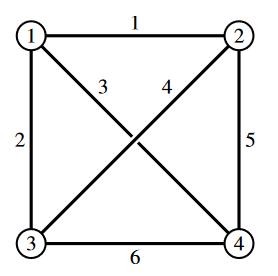
\includegraphics[width=\linewidth,keepaspectratio=true]{./Images/netzwerkzyklus.png}
	\end{minipage}%%% to prevent a space
	\begin{minipage}{0.3\textwidth}
		\begin{tabular}{ll}
			''von'' &= -1\\
			''nach'' &= +1
		\end{tabular}

		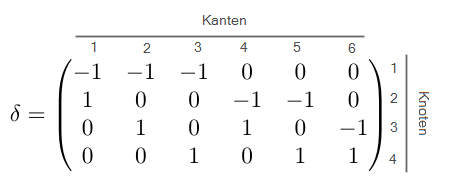
\includegraphics[width=\columnwidth]{./Images/netzwerkzyklus_matrix.png}
	\end{minipage}
\end{center}

\[\xrightarrow{Gauss} \begin{pmatrix}
	1 & 0 & 0 & -1 & -1 & 0 \\
	0 & 1 & 0 & 1 & 0 & -1 \\
	0 & 0 & 1 & 0 & 1 & 1 \\
	0 & 0 &0 &0 &0 &0 \\
\end{pmatrix}\]

\noindent Daraus liest man ab, dass drei Zyklen gebildet werden, die dadurch bestimmt sind, ob man die Kanten 4,5 oder 6 im Zyklus drin haben will oder nicht. 
 \[
 z_1 = \begin{pmatrix}
 	1 \\ -1 \\ 0 \\ \textbf{1} \\ 0 \\ 0
 \end{pmatrix} 
\qquad
z_2 = \begin{pmatrix}
	1 \\ 0 \\ -1 \\ 0 \\ \textbf{1} \\ 0
\end{pmatrix} 
\qquad
z_3 = \begin{pmatrix}
	0 \\ 1 \\ -1 \\ 0 \\ 0 \\ \textbf{1}
\end{pmatrix} 
\qquad
\]

\newpage

\subsection{Kamerageometrie}
\begin{wrapfigure}{r}{0.5\linewidth}
	\vspace{-10pt}
	\centering
	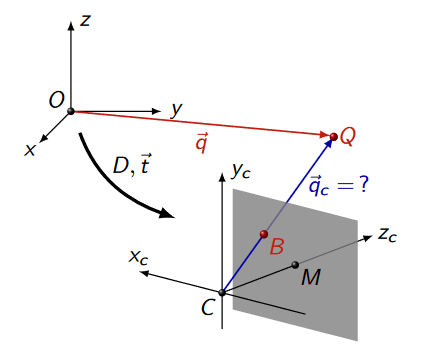
\includegraphics[height=10em]{./Images/kamera_geometrie.png}
\end{wrapfigure}

Um 3D Punkte von einem Welt-Koordinatensystem $O$ in ein Chip-Koordinatensystem zu übertragen (oder vica-versa), muss das Kamera-Koordinatensystem um $C$ Verschoben und mit Matrix $D$ gedreht werden. Nun liegen beide Koordinatensysteme übereinander. Die Kameramatrix $K$ kann nun eine Gerade $r_i$ finden, auf der der gesuchte 3D Punkt liegt. Meist sind mehrere Kameras in Verwendung, um die Position genauer mithilfe des \verweiseref{leastsquare} zu bestimmen

\subsubsection{Kameramatrix}
\begin{center}
	\begin{minipage}{0.2\textwidth}
		\[K = \begin{pmatrix}
			f & 0 & \frac{m_x}{2} \\
			0 & f & \frac{m_y}{2} \\
			0 & 0 & 1
		\end{pmatrix}\]
	\end{minipage}%%% to prevent a space
	\begin{minipage}{0.2\textwidth}
		$f$: Brennweite in Pixel \\
	    $m$: Chip-Grösse
	\end{minipage}
\end{center}

\subsubsection{Chip-Koordinaten berechnen}
Pixel-Position auf Chip berechnen von einem 3D Punkt.
\[ 
\underbrace{
	\begin{pmatrix}
		b_x \\ b_y \\ b_z = 1
	\end{pmatrix}}_{\tilde{b}\text{: Chip-Koordinaten}
}
= KD \cdot
\left(
	\underbrace{\begin{pmatrix}
		q_x \\
		q_y \\
		q_z
	\end{pmatrix}}_{\vec{q}\text{: Objekt 3D-Position}}
	-
	\underbrace{\begin{pmatrix}
		c_x \\
		c_y \\
		c_z
	\end{pmatrix}}_{\vec{c}\text{: Kamera-Position}}
\right)
\]

\noindent \textbf{Achtung:} Alle Komponenten von $\tilde{b}$ mit $\tilde{b}_z$ dividieren um homogener Bildpunkt zu erhalten.
$
b = \begin{pmatrix}
	\frac{\tilde{b}_x}{\tilde{b}_z} \\
	\frac{\tilde{b}_y}{\tilde{b}_z} \\
	\frac{\tilde{b}_z}{\tilde{b}_z}  = 1\\
\end{pmatrix}
$

\subsubsection{3D-Punkt triangulieren}
Zuerst den entsprechenden Stützvektor pro Kamera berechnen:
\[ 
\underbrace{
	\begin{pmatrix}
		r_x \\ r_y \\ r_z
\end{pmatrix}}_{\vec{r}\text{: Richtungsvektor}}
= (KD)^{-1} \cdot
\underbrace{
	\begin{pmatrix}
		b_x \\ b_y \\ 1
\end{pmatrix}}_{\tilde{b}\text{: Chip-Koordinaten}
}
\]

\noindent Die Gerade von jeder Kamera kann mit der Kamera-Position $c$ und dem berechneten Stützvektor $\vec{r}$ definiert werden:
\[
	\vec{p}_n = \vec{c} + t \cdot \vec{r}_n
\]

\noindent Die Matrix Gleichung aufstellen und mit \verweiseref{leastsquare} lösen:
\[
\underbrace{
	\begin{pmatrix}
		& & & & 0 \\
		& E & & -\vec{r}_1 & 0 \\
		& & & & 0 \\	
		& & & 0 & \\
		& E & & 0 & -\vec{r}_2 \\
		& & & 0 & \\
	\end{pmatrix}
}_{A}
\underbrace{
	\begin{pmatrix}
		x \\
		y \\
		z \\	
		t \\
		s 
	\end{pmatrix}
}_{\vec{x}}
=
\underbrace{
	\begin{pmatrix}
	    \\
		\vec{c}_1 \\
		\\	
		\\
	    \vec{c}_2 \\
		\\
	\end{pmatrix}
}_{\vec{b}}
\]